\section{Cluster Performance}
There are two important areas of measuring the performance of the cluster. The first being that as the size of the cluster is increased, the running time of the algorithms being executed should decrease as more computation is occurring in parallel. The second metric is that for a fixed-size cluster, the running time of the algorithms should only be affected by the size of the input.

\subsection{Size of Cluster}
Using Giraph, a runtime parameter for the job being submitted to the Hadoop cluster is to specify the number of workers to be included within the execution of the job. This allows us to analyse the running time of the jobs utilising differing amounts of computation power available from the cluster.

\subsubsection{Enron}
Using the Enron dataset as fixed size input, we are hoping to show that as the number of workers increase, the runtime of the algorithms decrease. From observations, the PageRank algorithm has shown to be one of the more time consuming algorithms, and as such has been chosen to perform analysis of the cluster.

\begin{figure}[htbp]%
\centering
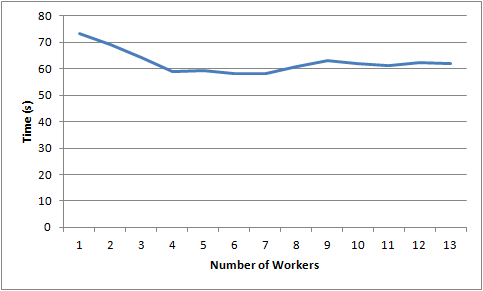
\includegraphics[]{./img/pagerank-enron-benchmark}%
\caption{Runtime of PageRank algorithm on Enron dataset with varying number of workers}%
\label{fig:enronbenchmark}%
\end{figure}

Figure \ref{fig:enronbenchmark} shows the running time of the PageRank algorithm on the Enron dataset consisting of 36692 nodes and 367662 edges. As expected, the running time of the algorithm initially decreases quite rapidly as the number of workers increases up to a fourth worker. There is minimal decrease in running time from the fourth to the seventh worker, followed by a jump after an eight worker is added. After this, the number of workers added do not affect the running time of the algorithm.

The longest running time, as to be expected, was with one worker. The shortest running time was with seven workers, again this is possibly to be expected as the cluster is in operation with seven slave nodes, so each node has an equal but small share of the original network. The running time does not decrease much from four to seven workers, most likely due to the increased network costs of having these extra workers offsetting the decrease in running time each worker will have from having less nodes to process.

After an eight worker is included, the running time then increases and stabilises just above the sixty second mark. This is most likely due to the nodes requiring to launch extra processes for the extra workers, which slows down the execution of workers on nodes with more than one worker.

\subsection{Size of Input}
The other metric which we want to analyse performance of the cluster is to observe how the running time for algorithms change as the size of the input is increased. To achieve this, we have opted to use seven workers for the Giraph jobs, as this has shown to produce the lowest running time for the PageRank algorithm on the Enron dataset. The algorithm which will be used for this analysis is also the PageRank algorithm, due it being a fairly time-consuming algorithm in relation to the other algorithms implemented.

We will make use of each of the datasets from Section \ref{sec:results_datasets} which we have been able to perform analysis on.

\begin{figure}[htbp]
  \centering \subfloat[]{\label{fig:inputsize-vertices-benchmark}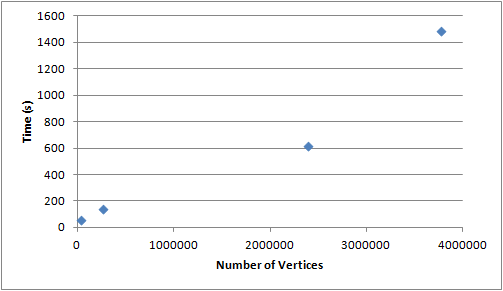
\includegraphics[width=0.45\textwidth]{./img/inputsize-vertices-benchmark}}
  ~ \subfloat[]{\label{fig:inputsize-edges-benchmark}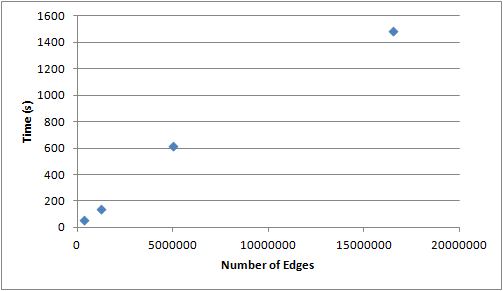
\includegraphics[width=0.45\textwidth]{./img/inputsize-edges-benchmark}}
  ~
  \caption{Running times of the PageRank algorithm on various size datasets using seven Giraph workers.}
  \label{fig:inputsize-benchmark}
\end{figure}

Figure \ref{fig:inputsize-benchmark} shows the results of running the PageRank on different size inputs. Figure \ref{fig:inputsize-vertices-benchmark} and Figure \ref{fig:inputsize-edges-benchmark} show that as the size of the input graphs are increased, then the cost to compute the PageRank values increases proportionally with the size of the input. For this benchmark, the PageRank algorithm was set to finish after 30 supersteps so that the dynamics of the networks were not influencing the runtime of PageRank too greatly.

\subsection{Conclusions}
We have shown that for current state of the cluster, with seven slave nodes
executing algorithms that the optimum running time for algorithms is achieved
when all seven of the slave nodes are used with one worker task assigned to
each. As the cluster grows, then it is quite likely that the optimum number of
workers will equal the size of the cluster. We have also shown that the system
is able to cope with a wide range of input sizes of graphs, which do noticeably
increase the running time of the algorithms, but with an increase in the size
of the cluster
